% Created 2023-11-26 Sun 20:39
% Intended LaTeX compiler: pdflatex
\documentclass[11pt]{article}
\usepackage[utf8]{inputenc}
\usepackage[T1]{fontenc}
\usepackage{graphicx}
\usepackage{longtable}
\usepackage{wrapfig}
\usepackage{rotating}
\usepackage[normalem]{ulem}
\usepackage{amsmath}
\usepackage{amssymb}
\usepackage{capt-of}
\usepackage{hyperref}
\usepackage[margin=0.5in]{geometry}
\author{Agustín Alejandro Mota Hinojosa}
\date{\today}
\title{Practice PL/SQL 5-1}
\hypersetup{
 pdfauthor={Agustín Alejandro Mota Hinojosa},
 pdftitle={Practice PL/SQL 5-1},
 pdfkeywords={},
 pdfsubject={},
 pdfcreator={Emacs 29.1 (Org mode 9.7)}, 
 pdflang={English}}
\begin{document}

\maketitle
\tableofcontents

\section{Vocabulary}
\label{sec:org441f954}

\begin{enumerate}
\item ROWTYPE Declares a record with the same fields as the cursor on which it is based
\item TYPE a composite data type consisting of a group of related data items stored as fields, each with its own name and data type
\end{enumerate}
\section{Try/Solve It}
\label{sec:org144a8c0}
\begin{enumerate}
\item Excecute following code and save it.
\begin{verbatim}
DECLARE
    v_dept_id DEPARTMENTS.DEPARTMENT_ID%TYPE;
    v_dept_name DEPARTMENTS.DEPARTMENT_NAME%TYPE;
    v_mgr_id DEPARTMENTS.MANAGER_ID%TYPE;
    v_loc_id DEPARTMENTS.LOCATION_ID%TYPE;
BEGIN
    SELECT department_id,department_name,manager_id,location_id
    INTO v_dept_id,v_dept_name,v_mgr_id,v_loc_id
    FROM DEPARTMENTS WHERE department_id = 80;
    DBMS_OUTPUT.PUT_LINE(v_dept_id || ' ' || v_dept_name || ' '
        || v_mgr_id || ' ' || v_loc_id);
EXCEPTION WHEN NO_DATA_FOUND THEN
    DBMS_OUTPUT.PUT_LINE('Department does not exist');
END;
\end{verbatim}
\begin{center}
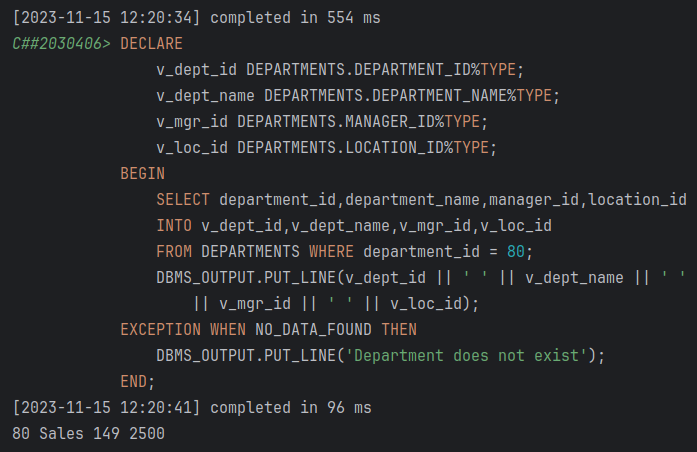
\includegraphics[width=.9\linewidth]{./resources/dbms_5-1.png}
\end{center}

\item Explain the advantage of using \texttt{\%ROWTYPE} to declare a record structure.

You don't need to specify the type of the table explicitly.
\end{enumerate}
\end{document}